\documentclass[12pt, notitlepage, final]{article} 

\newcommand{\name}{Vince Coghlan}

%\usepackage[dvips]{graphics,color}
\usepackage{amsfonts}
\usepackage{amssymb}
\usepackage{amsmath}
\usepackage{latexsym}
\usepackage{enumerate}
\usepackage{amsthm}
%\usepackage{nccmath}
\usepackage{setspace}
\usepackage[pdftex]{graphicx}
\usepackage{epstopdf}
%\usepackage[siunitx]{circuitikz}
\usepackage{tikz}
\usepackage{float}
%\usepackage{cancel} 
\usepackage{setspace}
%\usepackage{overpic}
\usepackage{mathtools}
\usepackage{listings}
\usepackage{color}
%\usepackage{gensymb}

\usetikzlibrary{calc}
\usetikzlibrary{matrix}
\usetikzlibrary{positioning}

\numberwithin{equation}{section}
\DeclareRobustCommand{\beginProtected}[1]{\begin{#1}}
\DeclareRobustCommand{\endProtected}[1]{\end{#1}}
\newcommand{\dbr}[1]{d_{\mbox{#1BR}}}
\newtheorem{lemma}{Lemma}
\newtheorem*{corollary}{Corollary}
\newtheorem{theorem}{Theorem}
\newtheorem{proposition}{Proposition}
\theoremstyle{definition}
\newtheorem{define}{Definition}
\newcommand{\column}[2]{
\left( \begin{array}{ccc}
#1 \\
#2
\end{array} \right)}

\newdimen\digitwidth
\settowidth\digitwidth{0}
\def~{\hspace{\digitwidth}}

\setlength{\parskip}{1pc}
\setlength{\parindent}{0pt}
\setlength{\topmargin}{-3pc}
\setlength{\textheight}{9.0in}
\setlength{\oddsidemargin}{0pc}
\setlength{\evensidemargin}{0pc}
\setlength{\textwidth}{6.5in}
\newcommand{\answer}[1]{\newpage\noindent\framebox{\vbox{{\bf ECEN 5018 Spring 2014} 
\hfill {\bf \name} \vspace{-1cm}
\begin{center}{Homework \#3}\end{center} } }\bigskip }

\DeclareMathOperator*{\argmin}{arg\,min}

%absolute value code
\DeclarePairedDelimiter\abs{\lvert}{\rvert}%
\DeclarePairedDelimiter\norm{\lVert}{\rVert}
\makeatletter
\let\oldabs\abs
\def\abs{\@ifstar{\oldabs}{\oldabs*}}
%
\let\oldnorm\norm
\def\norm{\@ifstar{\oldnorm}{\oldnorm*}}
\makeatother

\def\dbar{{\mathchar'26\mkern-12mu d}}
\def \Frac{\displaystyle\frac}
\def \Sum{\displaystyle\sum}
\def \Int{\displaystyle\int}
\def \Prod{\displaystyle\prod}
%\def \P[x]{\Frac{\partial}{\partial x}}
%\def \D[x]{\Frac{d}{dx}}
\newcommand{\PD}[2]{\frac{\partial#1}{\partial#2}}
\newcommand{\PF}[1]{\frac{\partial}{\partial#1}}
\newcommand{\DD}[2]{\frac{d#1}{d#2}}
\newcommand{\DF}[1]{\frac{d}{d#1}}
\newcommand{\fix}[2]{\left(#1\right)_#2}
\newcommand{\ket}[1]{|#1\rangle}
\newcommand{\bra}[1]{\langle#1|}
\newcommand{\braket}[2]{\langle #1 | #2 \rangle}
\newcommand{\bopk}[3]{\langle #1 | #2 | #3 \rangle}
\newcommand{\Choose}[2]{\displaystyle {#1 \choose #2}}
\newcommand{\proj}[1]{\ket{#1}\bra{#1}}
\def\del{\vec{\nabla}}
\newcommand{\avg}[1]{\langle#1\rangle}
\newcommand{\piecewise}[4]{\left\{\beginProtected{array}{rl}#1&:#2\\#3&:#4\endProtected{array}\right.}
\newcommand{\systeme}[2]{\left\{\beginProtected{array}{rl}#1\\#2\endProtected{array}\right.}
\def \KE{K\!E}
\def\Godel{G$\ddot{\mbox{o}}$del}

\onehalfspacing

\begin{document}

\answer{}

\textbf{1)} Recall BoS, Stag hunt, and Typewriter games from HW\#2. Compute \textit{all} of the
NE for these games (including mixed strategy NE).  \textit{Note that at the mixed strategy
equilibrium, both players are indifferent}.

BoS: I will use the game laid out as follows:
\begin{center}
  \begin{tabular}{r |c|c|}
    \multicolumn{1}{r}{}
    & \multicolumn{1}{c}{B}
    & \multicolumn{1}{c}{S}\\
    \cline{2-3}
    B & 2,1 & 0,0\\
    \cline{2-3}
    S & 0,0 & 1,2\\
    \cline{2-3}
  \end{tabular}
\end{center}

To find the NE I will construct a best response funcion as follows (note that it will be
symetric for player 2):
\[
  \underset{0\leq p\leq1}\max p(2\cdot q + 0\cdot(1-q)) + (1-p)(0\cdot q + 1\cdot(1-q))
\]
The maximizes value can be determined by seeing which coefficient is larger, we can come
up with the general best response as:
\[
  2q < (1-q) \text{ when } q < 1/3
\]
\[
  2q > (1-q) \text{ when } q > 1/3
\]

\[
B_{ROW}(q) = \left\{
   \begin{array}{lr}
     1 & q > 1/3\\
     0 & q < 1/3\\
     \text{[0,1]} & q = 1/3
   \end{array}
 \right.
\]
Similarily for player 2:
\[
B_{COL}(p) = \left\{
   \begin{array}{lr}
     1 & p > 2/3\\
     0 & p < 2/3\\
     \text{[0,1]} & p = 2/3
   \end{array}
 \right.
\]
The two pure NE occur when $(p,q) = (1,1)$ or $(p,q) = (0,0)$.  The mixed NE will occur
at $(p,q) = (1/3,2/3)$.  At this location, both players are indeed indifferent.  They dont
care what they play, but once they do play a different strategy, the other player will want
to change.

For Stag Hunt I will use the following payoff matrix:

\begin{center}
  \begin{tabular}{r |c|c|}
    \multicolumn{1}{r}{}
    & \multicolumn{1}{c}{Stag}
    & \multicolumn{1}{c}{Hare}\\
    \cline{2-3}
    Stag & 2,2 & 0,1\\
    \cline{2-3}
    Hare & 1,0 & 1,1\\
    \cline{2-3}
  \end{tabular}
\end{center}

We will again find the best response function:
\[
  \underset{0\leq p\leq1}\max p(2\cdot q + 0\cdot(1-q)) + (1-p)(1\cdot q + 1\cdot(1-q))
\]
\[
  2q < 1 \text{ when } q < 1/2
\]
\[
  2q > 1 \text{ when } q > 1/2
\]
Which tells us the best response for any player is:
\[
B_i(\omega) = \left\{
   \begin{array}{lr}
     1 & \omega > 1/2\\
     0 & \omega < 1/2\\
     \text{[0,1]} & \omega = 1/2
   \end{array}
 \right.
\]
The pure equilibria are $(1,1)$ and $(0,0)$ and the mixed equilibrium is $(1/2,1/2)$.

The Typewriter game has the following payoff matrix:
\begin{center}
  \begin{tabular}{r |c|c|}
    \multicolumn{1}{r}{}
    & \multicolumn{1}{c}{Dvorak}
    & \multicolumn{1}{c}{Standard}\\
    \cline{2-3}
    Dvorak & 3,3 & 0,0\\
    \cline{2-3}
    Standard & 0,0 & 1,1\\
    \cline{2-3}
  \end{tabular}
\end{center}
\[
  \underset{0\leq p\leq1}\max p(3\cdot q + 0\cdot(1-q)) + (1-p)(0\cdot q + 1\cdot(1-q))
\]
\[
  3q < 1-q \text{ when } q < 1/4
\]
\[
  3q > 1-q \text{ when } q > 1/4
\]
\[
B_i(\omega) = \left\{
   \begin{array}{lr}
     1 & \omega > 1/4\\
     0 & \omega < 1/4\\
     \text{[0,1]} & \omega = 1/4
   \end{array}
 \right.
\]

The pure equilibria are $(1,1)$ and $(0,0)$ and the mixed equilibrium is $(1/4,3/4)$.

\newpage
\textbf{2)} (a) Consider the following two player game.  Characterize the set of Nash equilibria,
Correnlated equilibria, and Course Correlated equilibria.
\begin{center}
  \begin{tabular}{r |c|c|}
    \multicolumn{1}{r}{}
    & \multicolumn{1}{c}{H}
    & \multicolumn{1}{c}{D}\\
    \cline{2-3}
    H & 0,0 & 6,1\\
    \cline{2-3}
    D & 1,6 & 4,4\\
    \cline{2-3}
  \end{tabular}
\end{center}

The pure Nash equilibria of this game are $HD$ and $DH$, since at these points niether player
has any reason to change.  There are also mixed strategy equilibria.  We can find this as we did
in the last example.

\[
  \underset{0\leq p\leq1}\max p(0\cdot q + 6\cdot(1-q)) + (1-p)(1\cdot q + 4\cdot(1-q))
\]
\[
  6(1-q) < 1+4(1-q) \text{ when } q < 1/2
\]
\[
  6(1-q) < 1+4(1-q) \text{ when } q > 1/2
\]
\[
B_i(\omega) = \left\{
   \begin{array}{lr}
     1 & \omega > 1/2\\
     0 & \omega < 1/2\\
     \text{[0,1]} & \omega = 1/2
   \end{array}
 \right.
\]

The correlated equilibria are a little harder to find.  We can start by assuming that the
signals will come with a probability for each action as follows:

\begin{center}
  \begin{tabular}{r |c|c|}
    \multicolumn{1}{r}{}
    & \multicolumn{1}{c}{H}
    & \multicolumn{1}{c}{D}\\
    \cline{2-3}
    H & $z_1$ & $z_2$\\
    \cline{2-3}
    D & $z_3$ & $z_4$\\
    \cline{2-3}
  \end{tabular}
\end{center}

We are going to first assum that player 1 is playing $H$, and we are going to also ignore
any normalization that occurs, since we are dealing with an inequality where the normalization
factors are the same.  We can this find:
\[
  P(a_2=H|a_1=H) = \frac{z_1}{z_1+z_2} \Rightarrow z_1
\]
\[
  P(a_2=D|a_1=H) = z_2
\]
Now we are looking at a comparrison of payoffs for player 1:
\[
  U(\text{obey}|a_1=H) = 6z_2
\]
\[
  U(\text{disobey}|a_1=H) = 1z_1 + 4z_2
\]
The equilibrium must therefor satisfy:
\[
  2z_2 \geq z_1
\]
Now we can assume that the signal for player 1 is $D$
\[
  P(a_2=H|a_1=D) = \frac{z_3}{z_3+z_4} \Rightarrow z_3
\]
\[
  P(a_2=D|a_1=D) = z_4
\]
\[
  U(\text{obey}|a_1=D) = 1z_3+4z_4
\]
\[
  U(\text{disobey}|a_1=D) = 6z_4
\]
The equilibrium must therefor satisfy:
\[
  z_3 \geq 2z_4
\]
For player two, symmetrically, $2z_3 \geq z_1$ and $z_2 \geq 2z_4$.  Additionally we know
that $z_1+z_2+z_3+z_4 = 1$.  From this we can derive the set of correlated equilibrium to
follow the following constraints:
\[
  z_1+z_2+z_3+z_4 = 1 \text{, } 2z_2 \geq z_1 \text{, } z_3 \geq 2z_4 \text{, } 2z_3 \geq z_1 \text{, and } z_2 \geq 2z_4
\]
Lets test our NE to make sure that every NE is also a correlated equilibria.  For $HD$, $z^a$
will look like $\{0, 1, 0, 0\}$.  This fits every one of the requirements.  $DH$ is going
to be the same due to symmetry.  The next one to test is $\{0, 1/2, 1/2, 0\}$.  This system
also fits the requirements set by the inequalities.

Coarse correlated equilibria are even harder to find.  We will assume the same probabitlity
distrobution $z^a$.  This means that the payoff for not opting out:
\[
  \sum_{a_{i}}U_i(a)z^a = 6z_2 + z_3 + 4z_4
\]
The payoff for opting out:
\[
  \sum_{a_{-i}}U_i(a_i',a_{-i})z_{-i}^{a_{-i}} = (z_1+z_3)1 + (z_2 + z_4)4
\]
This provides the inequality:
\[
  2z_2 \geq z_1
\]
Another payoff for opting out would be when $D$ is played:
\[
  \sum_{a_{-i}}U_i(a_i',a_{-i})z_{-i}^{a_{-i}} = (z_2+z_4)6
\]
This provides the inequality:
\[
  z_3 \geq 2z_4
\]
That means that a coarse correlated equilibria must satisfy the following requirements:
\[
  z_1+z_2+z_3+z_4 = 1 \text{, } 2z_2 \geq z_1 \text{, and } z_3 \geq 2z_4
\]
Note that these requirements are a subset of the requirements for a regular correlated
equilibrium.  Meaning that all regular correlated equilibrium and, by extension, all
Nash equilibrium, are also coarse correlated equilibrium. Note, however, that there are
correlated equilibria that is not a nash equilibria, and CCE that are not CE or NE.
This is the relationship that I will try and derive in part (b).

(b) Derive the relationship between Nash equilibria, correlated equililbria, and course
correlated quilibria and illustrate the results using a Venn diagram.  Prove all cases!
Give examples.  For example, give an example of a coarse correlated equilibrium that is
not a Nash equilibrium.


To do this I will first show that all NE are indeed CE.  Recall the definition of the
Nash equilibrium:
\[
  U_i(\alpha^*_i, \alpha^*_{-i}) \geq U_i(\alpha_i, \alpha^*_{-i})
\]
The system will also have mixed strategies represented as $\{z_1, z_2, z_3, z_4, \text{etc...}\}$ (where
$z_1 = p_n \cdot (1-q_1-q_2-...-q_n)$, etc...).  Since the payoff functions for these
mixed strategy equilibria are bournolli payoffs, they will look something like so:
\[
  U_i(\alpha_i,\alpha_{-i}) = z^{\alpha_1}\cdot U((\alpha_1)_i, (\alpha_1)_{-i}) + z^{\alpha_2}\cdot U((\alpha_2)_i, (\alpha_2)_{-i}) + ...
\]
This is where what is happening and my grasp of mathematical notation are at a standstill,
so let me try and explain this in plain english: The payoff of any mixed strategy is going
to be the sum of every payoff multiplied by the probability that it is played. Im going to
adopt the following notation to represent this:
\[
  U_i(a^*_i, a^*_{-i})z^*_{a_i} \geq U_i(a_i, a^*_{-i})z^*_{a_i}
\]

If we sum both sides of the inequality, the whole thing remains true, since you are summing
a bunch of things that are each know to be greater than the things summed on the right.
This means that the following holds true.
\[
  \sum_{a_-i}U_i(a^*_i, a^*_{-i})z^*_{a_i} \geq \sum_{a_-i}U_i(a_i, a^*_{-i})z^*_{a_i}
\]
Now exchanging terms with the ones used in the definition provided for CE we find:
\[
  \sum_{a_{-i}}U_i(a_i, a_{-i})z^{a_i,a_{-i}} \geq  \sum_{a_{-i}}U_i(a_i', a_{-i})z^{a_i,a_{-i}}
\]
Note that this is the definition of a CE, this means that all NE are CE.  Going backwards,
however, wont work, since if only one term in the sum is wrong, your sum may still hold
to the inequality, but that term wont.  In other words not every CE is a NE.

Now I will show that all CCE are CE with a similar process.

\[
  \sum_{a_{i}}\sum_{a_{-i}}U_i(a_i, a_{-i})z^{a_i,a_{-i}} \geq  \sum_{a_{i}}\sum_{a_{-i}}U_i(a_i', a_{-i})z^{a_i,a_{-i}}
\]
The left side is equivalent to the payoff in each square, the only part of the right side
that is dependent on $a_i$ is the probabilities.  This means that we can move the rest out
of the sum.
\[
  \sum_{a_{i}}U_i(a)z^a \geq \sum_{a_{-i}}U_i(a_i',a_{-i})\sum_{a_i}z^{a_i,a_{-i}}
\]
We will use the convinient definition of marginal probability that the professor provided:
\[
  z^{a_i,a_{-i}}_{-i} = \sum_{a_i}z^{a_i,a_{-i}}
\]
Substituting this in to our new equation gives us the following:
\[
  \sum_{a_{i}}U_i(a)z^a \geq \sum_{a_{-i}}U_i(a_i',a_{-i}) z^{a_i,a_{-i}}_{-i}
\]
Note that this is the exact definition of a CCE.  Meaning that by the same logic as previously
used, every CCE is a CE and by extension all NE must also be CCE.  This can be seen in a Venn
Diagram:

\begin{figure}[H]
\begin{center}
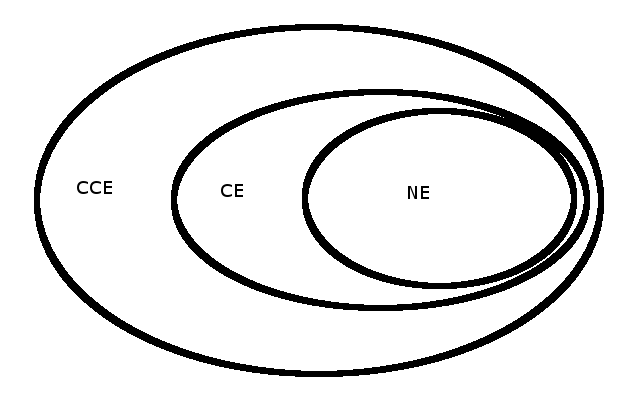
\includegraphics[width=10cm]{f1}
\end{center}
\end{figure}

Now for an example, We will take the same Hawk Dove example, as seen below:
\begin{center}
  \begin{tabular}{r |c|c|}
    \multicolumn{1}{r}{}
    & \multicolumn{1}{c}{H}
    & \multicolumn{1}{c}{D}\\
    \cline{2-3}
    H & 0,0 & 6,1\\
    \cline{2-3}
    D & 1,6 & 4,4\\
    \cline{2-3}
  \end{tabular}
\end{center}

We know the Nash equilibria to be $\{0,1,0,0\}$, $\{0,0,1,0\}$, and $\{0,1/2,1/2,0\}$. A
course correlated equilibria could, for example, be $\{0,0,3/4,1/4\}$.  This fits all of
the criteria found in part (a), meaning no player would not play this game given all other
players are in it.  This, however, could not be considered a CE since $z_2 \ngeq 2z_4$, and
one or more of the players would disobey any referee trying to implement this strategy. A
CE would look like $\{0,1/3,2/3,0\}$.  If players are told to play this, then they have no
incentive to deviate, This is clearly not a NE, since we only have three known NE.


\textbf{3)} A zero-sum game has a payoff (for the row player) given by
\[
  \begin{pmatrix}
    1 & 3 \\
    4 & 2
  \end{pmatrix}
\]
(a) Compute the security stratgies for both players using \textit{pure} actions, and
conclude that the game does not have a value in this case.

The row player's most secure move is to take the bottom strategy, since 2 is better
then getting 1.  The column player's secure strategy is the right column, since he
will at worst get 3.  The game does not have a value since 3 and 2 are different
numbers

(b) Repeat using \textit{mixed} strategies, and compute the value of the game.
The payoff in the case of the right column is:
\[
  1p+4(1-p)
\]
and in the left column
\[
  3p + 2(1-p)
\]
The maximin will occur when
\[
  1p+4(1-p) = 3p + 2(1-p) \Rightarrow 2(1-p) = 2p \Rightarrow p = \frac{1}{2}
\]
For player 2 the maximin will occur at:
\[
  q+3(1-q) = 4q + 2(1-q) \Rightarrow 1-q=3q \Rightarrow q = \frac{1}{4}
\]
We can find the value for player 1:
\[
  \frac{1}{2}3 + \frac{1}{2}2 = \frac{5}{2}
\]
Then for player 2:
\[
  \frac{1}{4}4 + \frac{3}{4}2 = \frac{5}{2}
\]
Since these are the same, we know that $(1/2,1/4)$ is a NE.


(c) Verify results using your Matlab function for Ficticious Play.

\end{document}
